\documentclass[]{article}
\usepackage{tikz}
\usepackage[ ]{graphicx}
\title{Revisão P1\\Linguagens Formais e Autômatos}
\author{Erickson G. Müller}
\date{}

\begin{document}
	\maketitle
	\section{Conteúdos}
		\begin{enumerate}
			\item Conceitos e linguagens: 
			\begin{itemize}
				\item Símbolo
				\item Alfabeto
				\item Cadeia
				\item Sentença 
				\item Concatenação
				\item Fechamento 
				\item Sufixo
				\item Prefixo
				\item Definição formal de gramática gerativa e derivação
				\item Tipos de gramáticas
			\end{itemize}
			\item Conceitos e linguagens
				Símbolo, alfabeto, cadeia, sentença, concatenação, fechamento, sufixo, prefixo. Definição
		\end{enumerate}
	\section{Teoria de Linguagens}
		Computabilidade; Algoritmos e decibilidade; Soluções algoritmica decidíveis e indecidíveis. Processadores de linguagens (tradutores e interpretadores).
		
		Para problemas computáveis podemos construir uma solução algoritmica que poderá ou não ter um resultado. Caso esse algoritmo não tenha um retorno, será considerado um algoritmo indecidível.
		
		Esse conjunto de cadeias pode ser formado pela concatenação de símbolos que pertence ao alfabeto da linguagem.
		
		Os processadores de linguagem verificam se a cadeia de símbolos \textbf{pertence} à linguagem. Os processadores de linguagens são soluções algoritmicas para \textbf{problemas decidíveis}. São divididos em tradutores e interpretadores.
		
		Os processadores de linguagens podem fazer transformações de linguagens de mesmo nível, podem passar de uma linguagem de código de uma máquina para outra máquina.
		
		Tradutores recebem uma entrada chamada de fonte, fazem o processamento e resultam um objeto.
%		\begin{tikzpicture}
%			\node (processo) [draw, ellipse] {processamento};
%			\node (fonte) [left=of processo] {fonte};
%			\node (objeto) [right=of processo] {objeto};
%			\draw [->] (fonte) -- (processo);
%			\draw [->] (processo) -- (objeto);
%		\end{tikzpicture}

		Nem todas as cadeias do fechamento do alfabeto são sentenças, todas as sentenças pertencem ao fechamento do alfabeto
		
		\textbf{Gramática:} Conjunto de regras que descreve como as cadeias podem ser montadas e quando elas são válidas.
		
		Sentença é toda cadeia de símbolos que pertence à linguagem.
		
		Aplicando as regras da gramática, teremos sempre uma \textit{cadeia ou sentença} %não sei qual dos dois
		\begin{center}
		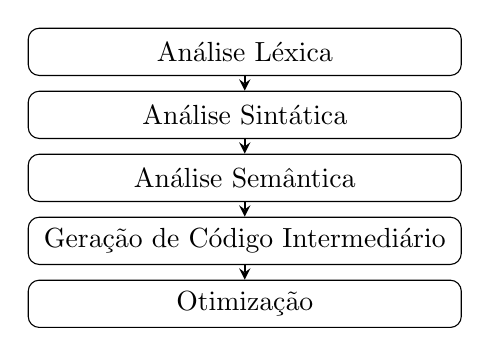
\begin{tikzpicture}[node distance=0.8cm, auto]
\tikzstyle{bloco} = [rectangle, rounded corners, minimum width=5.5cm, minimum height=0.6cm,text centered, draw=black]
\tikzstyle{seta} = [thick,->,>=stealth]

\node [bloco] (lexica) {Análise Léxica};
\node [bloco, below of=lexica] (um) {Análise Sintática};
\node [bloco, below of=um] (dois) {Análise Semântica};
\node [bloco, below of=dois] (tres) {Geração de Código Intermediário};
\node [bloco, below of=tres] (quatro) {Otimização};

\draw [seta] (lexica) -- (um);
\draw [seta] (um) -- (dois);
\draw [seta] (dois) -- (tres);
\draw [seta] (tres) -- (quatro);

\end{tikzpicture}
\end{center}

		Análise léxica faz o tratamento de erros, reconhecimento do tipo da variável através do identificador

		Faz parte da saída da análise léxica uma estrutura chamada de fita que pertence o identificador dos tokens, essa fita é a entrada da análise sintática. O final dessa fita é um símbolo de final de sentença. 

		Análise sintática faz a análise da sentença  usando o identificadores das cadeias que foram validadas na análise léxica. A sentença é avaliada através da concatenação de identificadores em uma determinada ordem.
		
		A análise semântica verifica  o tipo dos siímbolos e como estão sendo utilizados.
		
		A geração de Código intermediário passa a sentença para código assembly.
		
		
		\includegraphics[scale=0.1]{images/aula-1.png}
\end{document}
